\documentclass{standalone}
\usepackage{tikz}

\usetikzlibrary{hobby,arrows.meta}

\begin{document}
    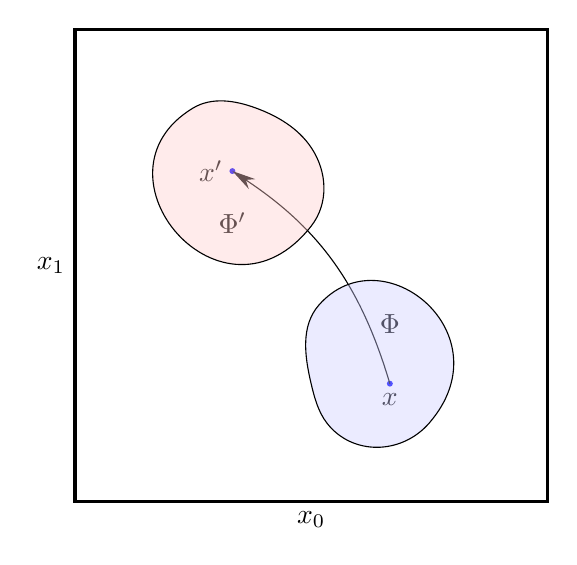
\begin{tikzpicture}
        \draw[very thick] (-3,-3) rectangle (3,3);
        \node [below] at (0,-3) {$x_0$};
        \node [left] at (-3,0) {$x_1$};
        \node [below] at (1,-1.5) {$x$};
        \node [left] at (-1,1.2) {$x'$};
        \node [below] at (1,-0.5) {$\Phi$};
        \node [below] at (-1,0.8) {$\Phi'$};
        \filldraw[blue] (1,-1.5) circle (.03);
        \filldraw[blue] (-1,1.2) circle (.03);
        \draw [-{Stealth[length=3mm, width=1.5mm]}] (1,-1.5)[bend right=20] to (-1,1.2);
        \filldraw[fill=blue!20,fill opacity=0.4] (1.5,-2) to [closed,curve through={(0.1,-0.5) (0,-1.5)}] (0.2,-2);
        \filldraw[fill=red!20,fill opacity=0.4] (-1.5,2) to [closed,curve through={(0,0.5) (0,1.5)}] (-0.7,2);
    \end{tikzpicture}
\end{document}